\section{Energie und Arbeit}
\subsection{verschiedene Energieformen}
\begin{description}
	\item[kinetische Energie] BILD
		\[ E_{\text{kin}} = \frac{1}{2} m v^2 \]
	\item[potentielle Energie] BILD
		\[ E_{\text{pot}} = mgh \]
	\item[Federenergie] BILD
		\[ E_{\text{pot}} = \frac{1}{2} D x^2 \]
\end{description}

\subsection{Arbeit}
Umwandlung einer Energieform in die andere via Kräfte \\
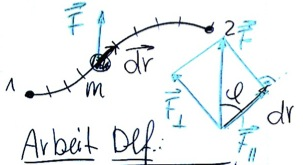
\includegraphics{Bild68} \\
\begin{def*}[ note = Arbeit , index = Arbeit ]
	\[
		\begin{split}
			\dd W
				&= \vec{F} \cdot \vec{\dd r} \\
				&= F \cdot \dd r \cdot \cos \phi \\
				&= F_{||} \cdot \dd r
		\end{split}
		\intertext{Gesamte Arbeit}
		W_{1 \rightarrow 2} = \int_1^2 \vec{F} \cdot \vec{\dd r} \\
		[ W ] = \si{\newton\metre} = \si{\joule} \text{ (Joule)}
	\]
\end{def*}
\begin{bsp*}[ note = Arbeit zum Spannen einer Feder ]
	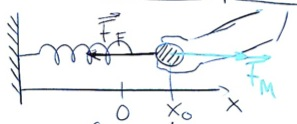
\includegraphics{Bild69} \\
	ganz langsam!
	\[
		\implies E_{\text{kin}} = 0 \\
		\vec{F_M} = -\vec{F_F} \\
		F_F = -D \cdot x \\
		\text{Arbeit der Hand } W_{0 \rightarrow x_0} = \int_0^{x_0} \vec{F_M} \cdot \vec{\dd r} \\
		W_{0 \rightarrow x_0} = \int_0^{x_0} F_M \cdot \dd x = \int_0^{x_0} D \cdot x \dd x = \left. \frac{1}{2} D x^2 \right|_0^{x_0} = \frac{1}{2} D x_0^2
	\]
\end{bsp*}

\begin{rep*}[ note = Hydrostatik ]
	Druckverteilung in Flüssigkeiten:
	\[ p(z) = p_0 + \rho_{\text{Fl.}} g z \]
	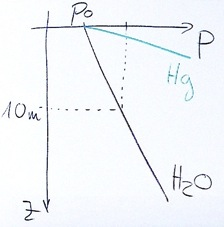
\includegraphics{Bild70}
	\begin{folge}[ note = Auftrieb ]
		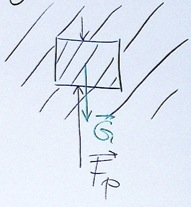
\includegraphics{Bild71}
	\end{folge}
	Zentifuge:
	\[ p(r) = p_0 + \frac{1}{2} \rho_{\text{Fl.}} \omega^2 ( r^2 - r_0^2 ) \]
	Energie und Arbeit: \\
	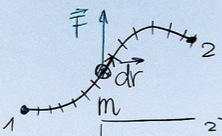
\includegraphics{Bild72} \\
	Arbeit:
	\[ W_{1 \rightarrow 2} = \int_1^2 \vec{F} \cdot \vec{\dd r} \]
	z.B. Spannen einer Feder
	\[ W_{0 \rightarrow x_0} = \frac{1}{2} D x_0^2 \]
\end{rep*}

\subsection{Energie und Energieerhaltungssatz}
\subsubsection{Situation}
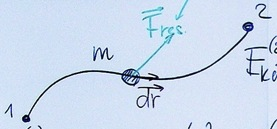
\includegraphics{Bild73} \\
$W_{1 \rightarrow 2}$: Arbeit sämtlicher an $m$ angreifender Kräfte ($\vec{F_{\text{res}}}$)
\[ W_{1 \rightarrow 2} = \int_1^2 \vec{F_{\text{res}}} \cdot \vec{\dd r} \]
\begin{satz*}[ note = Energiesatz , index = Energie satz Satz , indexformat = {1!~.2 3!1~} ]
	\[ W_{1 \rightarrow 2} = E_{\text{kin}}^{(2)} - E_{\text{kin}}^{(1)} \]
\end{satz*}
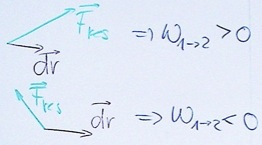
\includegraphics{Bild74}
\begin{bsp*}[ note = Bremsung ]
	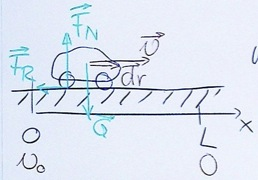
\includegraphics{Bild75}
	\[
		\vec{F_{\text{res}}} = \underbrace{\vec{G} + \vec{F_N}}_{0} + \vec{F_R} \\
		W_{1 \rightarrow 2} = -\int_0^L F_R \dd x = -\int_0^L \mu_G m g \dd x = -\mu_G m g L = 0 - \frac{1}{2} m v_0^2 \\
		L = \frac{v_0^2}{2 \mu_G g}
	\]
\end{bsp*}

\subsubsection{Situation Energieerhaltungssatz}
Bewegungen unter Einfluss \textbf{konservativer Kräfte} (z.B. Gewichtskraft , Federkraft ) \\
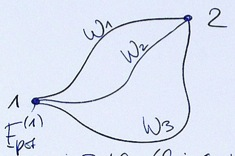
\includegraphics{Bild76} \\
$W_1$: Arbeit der \textbf{konservativen} Kraft \\
\textbf{konservativ}: $W_1 = W_2 = W_3$ ; $W_{1 \rightarrow 2}$ ist unabhängig vom Weg \\
$\implies$ zwei Zahlen (bei Ort 1,2 genügen) \\
$\implies$ $W_{1 \rightarrow 2}$ hängt nur von Lage ab
\begin{def*}[ note = potentielle Energie , index = potentielle Energie , indexformat = {2!1~}]
	\[ E_{\text{pot}}^{(2)} - E_{\text{pot}}^{(1)} = - W_{1 \rightarrow 2} \]
\end{def*}
\begin{bsp*}
	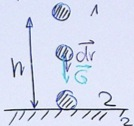
\includegraphics{Bild77}
	\[
		E_{\text{pot}}^{(1)} = mgh \\
		E_{\text{pot}}^{(2)} = 0 \\
		W_{1 \rightarrow 2} = \int_1^2 mg \dd z = mgh
		\intertext{Also:}
		0 - mgh = -mgh \quad \checkmark
	\]
\end{bsp*}
\begin{satz*}[ note = Energie-Erhaltungssatz , index = Energie-Erhaltungs satz Satz , indexformat = {1!~.2 3!1.~} ]
	\[ E_{\text{tot}} = E_{\text{kin}} + E_{\text{pot}} = \text{ konst.} \]
\end{satz*}
\begin{bsp*}[ note = Berg- \& Talbahn ]
	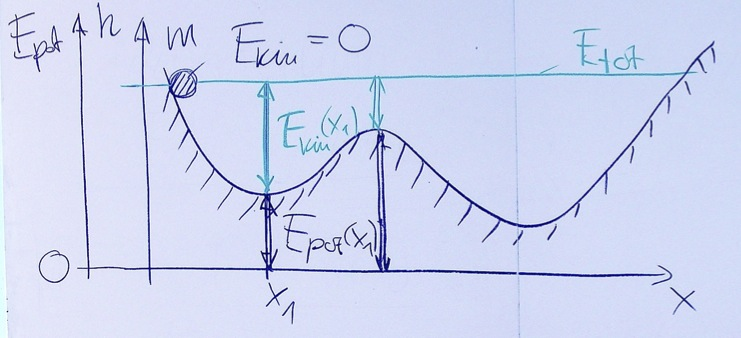
\includegraphics[ width = \textwidth ]{Bild78}
\end{bsp*}